%!TEX root = ../thesis.tex

\section{追従フェーズ}

  追従フェーズでは,学習フェーズで学習したモデルを活用し,\figref{Fig:okada_route}に示す経路(学習フェーズと同じ経路)でテストを行う.この際,引き紐は不要であり,代わりに深層学習器に画像が入力され,その出力がロボットの行動となる.つまり,学習フェーズで利用された引き紐によるルールベース制御器の出力ではなく,カメラ画像に基づく深層学習器の出力がロボットの行動になる.

  \vspace{1.5cm}

  \begin{figure}[h]
    \centering
    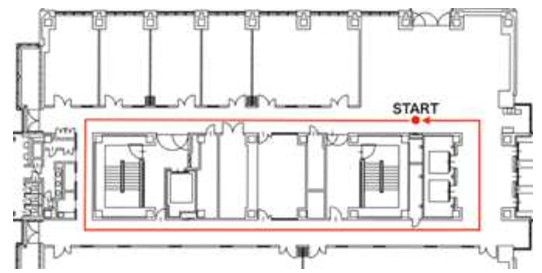
\includegraphics[keepaspectratio, scale=1.2] {images/pdf/okada_route}
    \caption[Target trajectory that the operator walks]{Target trajectory that the operator walks (source: \cite{okada})}
    \label{Fig:okada_route}
  \end{figure}

\newpage